\documentclass[10pt,a4paper,final,onecolumn]{article}
%\usepackage{fontspec}
%\defaultfontfeatures{Mapping=tex-text}
%\usepackage{xunicode}
%\usepackage{xltxtra}
%\setmainfont{???}

\usepackage{amsmath}
\usepackage{amstext}
\usepackage{array}
\usepackage{amssymb}
\usepackage{graphicx}
\usepackage{booktabs}
\usepackage{natbib}
\usepackage{lscape}

\newcolumntype{L}{>{$}l<{$}} % math-mode version of "l" column type

\author{Fennell \textit{et al.}}
\title{High-level simulation of future multispectral imagery from the proposed TreeView satellite. v1.3}

\begin{document}
\maketitle
\begin{abstract}
This document describes the early work carried out for the development of a simulation-evaluation pipeline for earth orbit multispectral imagery. A description of the pipeline is presented and example outputs.
\end{abstract}
\section{Introduction}
% From proposal Docs
The TreeView project proposes a novel satellite solution for climate action that will drive a revolution in ‘Precision Forestry’ –- the use of advanced technologies for a more granular data capture and management. Forests are often considered large, remote areas that require low maintenance during their lifetime and can be managed in homogeneous units called forest stands. But new political, environmental, social and commercial drivers necessitate a more diverse approach of mixed species and smaller scale planting. Individual trees are the fundamental unit of these resources, and the target of TreeView. 

\subsection{Work Package 2000: Science Requirements}
Current work (Q4 2020) focuses on the need to constrain the engineering design with understanding of the likely measurements that will be made with the proposed system. In order to do this, both a simulation methodology and a set of relevant performance metrics must be adopted, such that different combinations of band-pass filter and sensor characteristics can be evaluated for different geographically-relevant atmospheric conditions.

In designing the work the following considerations were made:

\begin{enumerate}
\item As this project relates specifically to the measurement of single trees (as opposed to forest stands), tree stands and individual isolated trees of various sizes will both be considered when designing performance metric experiments
\item Due to the limited knowledge of the likely system architectures at this stage in the development process, a high-level approach will be taken to simulation of synthetic images with assumptions made about the likely distributions and properties of noise at different stages in the simulation.
\item The range of possible spectral sensitivities will be limited to what is feasible with a silicon detector, and observable through standard glass optics ($\lambda \approx 400 - 900$ nm).
\item The simulation pipeline is designed using Dask/Python as it is (i) Open Source (and so easily verified, reviewed and tested by any research group) and (ii) a natively parallel environment for efficient, scalable computation.
\end{enumerate}
 
\subsection{Simulation of a line-scanning sensor}
A line-scanning Time Delay Integration (TDI) Charged Metal Oxide Silicon (CMOS) sensor is the only likely sensor suitable for purpose and so this work focuses on the simulation only of this class of sensor.

\section{Methods}
This section details the tools and methodologies used for each stage in the simulation/evaluation pipeline.
\subsection{Imagery Collection}
Hyperspectral aerial imagery from the project partners 2ExcelGeo have been used as the main reference data for these simulations. The relevant datasets from the aerial collect were the HySpex VNIR covering a spectral range covering the 400-900 nm band and at a ground sampling distance of $0.33 m pixel^{-1}$ - much higher spatial and spectral resolution than the proposed mission. Imagery have been collected over a number of UK cities including Milton Keynes and Birmingham. Time sequences (multiple images of the same ground area) have been collected over some areas and will be made available to this team within the current project.

The measured at-sensor radiance is converted to a reflectance value through an  atmospheric correction model implemented in ENVI software (QUAC [ref needed]). This is carried out by the data providers (2ExcelGeo). The QUAC method is based on the use of lookup tables of pure endmember reflectances and their corresponding radiance under known solar conditions. The ill-posed problem is then treated as a spectral-unmixing of known endmembers. It is favoured for it's low computation demand, however there is some concern that the approach may introduce spectral artefacts to the imagery that are hard to quantify and studies have shown worse performance than conventional radiative transfer model inversion methods such as FLAASH [citation needed]. More work needed to understand if a more rigorous atmospheric approach is needed for these data.

\subsection{Simulation}
\subsubsection{Definitions}
\begin{tabular}{Ll}
\toprule
Symbol & Definition \\ 
\midrule
A_{pix} & Area of pixel \\
a_{fov} & Angular Field of View\\
CONU & Column Offset Non-Uniformity \\
d_{swath} & Swath width\\
d_{altitude} & Altitude of sensor\\
D & Diameter of front optic \\
DN & Digital Number \\
DSNU & Dark Signal Non-Uniformity \\
FWHM & Full Width at Half Maximum\\
FWC & Full Well Capacity\\
f & Focal length\\
g(x^{\prime}, y^{\prime}) & Spatial degradation kernel function \\
G_{ADC} & ADC Gain \\
G_{SN} & Sense node gain \\
hc & $1.98644586\times 10^{-25}$\\
k_{dark} & coefficient of non-uniformity in dark signal \\
k_{light} & coefficient of non-uniformity in photon response \\
k_{offset} & coefficient of column amplifier non-uniformity \\
\lambda & Wavelength ($nm$)\\
\Lambda & Poisson parameter \\
L_{e, \Omega} & Radiant Energy ($W m^{-2} sr^{-1}$)\\
L_{\Omega} & Radiant Photon flux ($m^{-2} sr^{-1} s^{-1}$)\\
\nu_{y} & Line read frequency\\
\bar{N}_{p}  & Mean photons per pixel per cycle \\
\Omega & Solid angle\\
PRNU & Photon Response Non-Uniformity \\
R(\lambda) & Spectral reflectance\\
sr & Steradian \\
s\prime & Rear optic-sensor separation \\
\sigma & Standard deviation \\
t_{eff} & effective integration time \\
T(\lambda) & Spectral transmittance \\
V_s & CMOS sensor voltage \\
V_{ADC} & ADC reference voltage \\
V_{SN} & CMOS reference voltage \\



 
\bottomrule
\end{tabular} 
\subsubsection{Reflectance to at-sensor radiance}
In broad terms, the purpose of the atmospheric simulation is to map from ground reflectance ($R$) to an at-sensor radiance ($L_{e, \Omega}$):

\begin{equation}
R(\lambda) \rightarrow L_{e, \Omega} (\lambda)
\end{equation}

Established radiative transfer modelling approaches were used in the simulation. Primarily, the 6SV [ref needed] code from NASA was used to convert the measured ground reflectance to at-sensor radiance outside the atmosphere. The code is considered a medium-complexity, line-by-line approach and is used for atmospheric correction of MODIS data. For practical implementation reasons, the 6SV code (a FORTRAN library accessed via the Py6S bindings) has been used to generate Lookup Tables (LUTs) for a limited range of parameter values.

In the first stages, the following approximations are proposed:
\begin{enumerate}
\item The satellite observes each pixel in space, at nadir. If the centre of the image plane is assumed to be directly beneath the satellite's orbital path, then the inaccuracy introduced by this approximation increases towards the edges of the image plane. This is a reasonable approximation for a narrow field-of-view, high resolution device as proposed. 
\item The atmospheric optical thickness will be set at a range typical of the UK. All test data is of UK locations and the UK's climatic conditions are quite challenging for optical imaging. This is therefore a useful starting point for simulation.
\item All individual pixels in the imagery array will be considered as independent homogeneous lambertian diffusers for the purpose of the 6SV simulation. As such, the spatial response function is handled at a later stage in the pipeline.
\item The simulation is evaluated for all wavelengths between 
\end{enumerate}

\subsubsection{Radiant energy to radiant quanta}
The top-of-atmosphere apparent radiance is converted from energy ($L_{e,\Omega}$) to quantity of photons ($L_{\Omega}$) using the Planck-Einstein relation:
\begin{equation}
L_{\Omega}(\lambda) = L_{e,\Omega}(\lambda)\frac{\lambda}{hc}
\end{equation}

\subsubsection{Application of bandpass response functions}
For every band, the bandpass transmittance is multiplied element-wise by the radiant flux and integrated w.r.t. wavelength
\begin{equation}
L_{\Omega}(band)= \int_{400}^{900}(L_{\Omega}(\lambda)T_i(\lambda))~d\lambda
\end{equation}

where $T_{band}$ is the transmission spectrum of a bandpass filter

\subsubsection{Spatial resampling}
The spatial response function takes into account atmospheric blurring, optical imperfections, motion blur, etc. of the entire system.

To convert from the ground plane to image plane, the integrated radiant flux ($L_{\Omega}(band)$) are separately convolved with the spatial response function, $g(x^\prime,y^\prime)$.
\begin{equation}
L_{\Omega}(band, x, y) = g(x^\prime, y^\prime) * L_{\Omega}(band, x^\prime, y^\prime)
\end{equation}
where $x, y$ are simulated sensor spatial position indices and $x^{\prime}, y^{\prime}$ are input array position indices.

In the absence of more information about the optical properties, the spatial response function ($g(x^\prime, y^\prime)$) has been approximated as a 2D gaussian with parameters derived empirically. An example of this using the Sentinel 2 Point Spread Function estimated the 10m ground sampling distance Sentinel 2 bands to have a Full Width at Half Maximum (FWHM) of 22.08 m and this ratio was used for preliminary estimates of different ground sampling distances.

The FWHM is converted to pixel-plane sigma:

\begin{equation}
\sigma_{xy} = \frac{(FWHM/2.355)}{dx}
\end{equation}

where $dx = dy$

and used to generate the gaussian kernel:

\begin{equation}
g(x^\prime, y^\prime) =\exp \left[-\left({\frac {(x^\prime-x_{0}^\prime)^{2}}{2\sigma _{xy}^{2}}}+{\frac {(y^\prime-y^\prime_{0})^{2}}{2\sigma _{xy}^{2}}}\right)\right]
\end{equation}

After convolution, the new array is then resampled by taking the local mean over a subset of cells representing the area of one sensor pixel.

\subsubsection{Radiance to sensor flux density}
The at-satellite radiance ($L_{\Omega}(band)$) is in units of photons per steradian per ground area per second ($sr^{-1} m^{-2} s^{-1}$) and so requires conversion to at-sensor flux density ($E$) ($m^{-2} s^{-1}$). When treated as a thin lens problem (in the absence of optic specifics) the irradiance at a position($\textbf{x}$) on the sensor is calculated as the solid angle subtended by the lens. We follow the interpretation by \cite{Sato1999} to show that sensor irradiance is linearly related to radiance and dependent on the diameter of the front optic ($D$), focal length ($f$) and the pixel-lens normal offset angle ($\alpha$):
\begin{equation}
E(band, x, y) = L_{\Omega}(band) \frac{\pi}{4} \left(\frac{D}{f}\right)^{2} \cos^4 \alpha(x,y)
\label{eqn1}
\end{equation}

The angular field of view ($a_{fov}$) is calculated from the swath width ($d_{swath}$) and sensor altitude ($d_{altitude}$):

\begin{equation}
a_{fov} = 2\cdot \tan^{-1}\frac{0.5\cdot~d_{swath}}{d_{altitude}}
\end{equation}

The focal length ($f$) is calculated assuming the optic will be focused near infinity and so, from the thin lens equation, the distance between rear optic and lens ($s\prime$) is approximately equal:

\begin{equation}
\frac{1}{s^\prime} + \frac{1}{\infty} = \frac{1}{f} \approx \frac{1}{s^\prime}
\end{equation}

and so the angular field of view ($a_{fov}$) and sensor width ($d_{sensor}$) are used to calculate the required focal length:

\begin{equation}
f= \frac{d_{sensor}}{\tan a_{fov}}
\end{equation}

As focal length is expected to be very large due to the distance from target and narrow swath needed to achieve target ground sampling distances, the $\cos^4\alpha(x, y)$ term will have a minimal effect on the simulation and so is omitted for computational simplicity

\subsubsection{Effective Integration Time}
The Time Delay Integration sensor uses a column of pixels to collect photons from the same point in space as the sensor passes over. This increases the effective integration time ($t_{eff}$), calculated from the line rate ($\nu_{y}$) and the number of rows in a TDI pixel sub-array ($n$).

\begin{equation}
t_{eff} = \frac{n}{\nu_{y}}
\end{equation}

\subsubsection{Flux density to pixel quantity}
To convert from pixel flux density ($E$) to pixel photon count:

\begin{equation}
\bar{N}_{p}(x, y, band) =  E(band, x, y) t_{eff} A_{pix}
\end{equation}

where $t_{eff}$ is integration time and $A_{pix}$ is the area of the pixel. The quantity $\bar{N}_{p} $  describes the mean number of photons striking a pixel in any given integration cycle.

\subsubsection{Photon shot noise}
The photon count at the sensor can be expressed as a Poisson process such that the $\Lambda$ coefficient of each process is the observed count for a given pixel

\begin{equation}
N_{p}(x, y, band) \sim Poisson(\Lambda)
\end{equation}

Where the estimated photon quantity at each pixel, $\bar{N}_{p}(x, y, band) $ is the $\Lambda$ coefficient for each distribution.

\subsubsection{Photon to electron}
To convert from photon to electron, given a known sensor quantum efficiency:

\begin{equation}
N_{light}=  round(N_{p}(x, y, band) \cdot \bar{Q}_{E,band})
\end{equation}

where $\bar{Q}_{E,band}$ is the weighted mean of the quantum efficiency in each band:

\begin{equation}
\bar{Q}_{E, band} = \sum_{\lambda=300}^{900} Q_{E}(\lambda) \left(\frac{T_{band}(\lambda)}{\int_{300}^{700} T_{band}(\lambda) d\lambda}\right)
\end{equation}

\subsubsection{Photon Response Non-Uniformity}
The response of the sensor varies from pixel to pixel and so this non-uniformity can be treated as a zero mean gaussian distribution (i.e. the mean effect over the whole sensor is zero)

\begin{equation}
PRNU \sim \mathcal{N}(0, \sigma_{PRNU}^{2})
\end{equation}

where

\begin{equation}
\sigma_{PRNU} = k_{light}
\end{equation}
 where $k_{light}$ is the coefficient of photon response non-uniformity provided by the manufacturer.
 
\subsubsection{Dark current estimation}
The dark current density ($j_{dark}$) is measured at a constant temperature ($20^{\circ} C$) and so the mean signal per sub-pixel array is estimated as

\begin{equation}
\bar{N}_{dark} = 6.242 \times 10^{18} \cdot j_{dark} \cdot t_{eff} \cdot A_{pix}
\end{equation}

\subsubsection{Dark Signal Non-Uniformity}
The dark signal will vary pixel to pixel and so this is accounted for with a zero-mean log-gaussian distribution (i.e. the mean effect over the whole sensor is zero). This has been experimentally shown to be suitable of integration times of less than 100 seconds

\begin{equation}
DSNU \sim Log\mathcal{N}(0, \sigma_{DSNU}^{2})
\end{equation}

where

\begin{equation}
\sigma_{DSNU} = \bar{N}_{dark} \cdot t_{eff} \cdot k_{dark}
\end{equation}

where $k_{dark}$ is the coefficient of non-uniformity, provided by the manufacturer.

\subsubsection{Dark current shot noise}
The dark current is expected to follow a Poisson distribution and so 

\begin{equation}
N_{dark}(x, y, band) \sim Poisson(\Lambda)
\end{equation}

Where the estimated photon quantity at each pixel, $\bar{N}_{dark}(x, y, band) $ is the $\Lambda$ coefficient for each distribution.

\subsubsection{Read Noise}
The read noise is estimated from measured values and is assumed independent of signal. It is modelled as a zero-mean gaussian

\begin{equation}
N_{read} \sim \mathcal{N}(0, \sigma_{read}^{2})
\end{equation}

\subsubsection{Total charge}
The signals are added
\begin{equation}
N = N_{dark} + (N_{dark} \cdot DSNU) + N_{light}
+ (N_{light} \cdot PRNU) + N_{read}
\end{equation}

This value is truncated at the full well capacity of the pixel sub-array.


\subsubsection{Charge to voltage}
The charge collected during an integration cycle is then converted to a voltage by the column amplifiers

\begin{equation}
V_s = V_{SN}(N \cdot G_{SN})
\end{equation}
where $V_{SN}$  is the reference voltage (V) and $G_{SN}$ is the sense node gain ($V/e^{-}$).

The Full Well Capacity ($FWC$) can be used to define $G_{SN}$ to cover the full charge handling capacity of the sensor:

\begin{equation}
G_{SN} = \frac{V_{SN}}{FWC}
\end{equation}

\subsubsection{Conversion to Digital Number}
The amplified voltage is then converted to a digital number (DN) the Analogue-Digital Converter (ADC)

\begin{equation}
DN = DN_{max}~\frac{V_s}{V_{ADC}}
\end{equation}
where $V_{ADC}$  is the Analogue-Digital Converter reference voltage.

The resulting array is truncated between zero and the maximum DN value ($DN_{max}$) to simulate non-detection and clipping behaviours.

\subsubsection{Conversion to reflectance}
For testing and evaluation purposes, the pipeline is used to generate a sensor response for a 100\% reference image (i.e. all atmospheric and sensor parameters are known \textit{a priori}). The image signal is then divided by reference signal to produce the estimate of reflectance at surface level.

\begin{equation}
\widehat{R}(\lambda)= \frac{DN}{DN_{100}}
\end{equation}

Noisy reference spectra can easily be generated by replacing fixed parameters with a distribution from which instances are sampled, for example to explore effect of uncertainties in Atmospheric Optical Thickness (AOT) measurement.

\section{Evaluating Performance}
Performance metrics for a given sensor-atmosphere parameterisation can be divided into classification and parameter estimation metrics

\subsection{Signal-to-Noise Ratio}
SNR was calculated by generating 10,000 instances of each input radiance and measuring the properties of the distribution generated. The definition used for SNR was:
\begin{equation}
    SNR = \frac{\mu}{\sigma}
\end{equation}
for the mean ($\mu$) and standard deviation ($\sigma$) of the output distribution.

\subsection{Parameter estimation}
A spectral index (defined by narrowband wavelength or wavelength ranges) is first estimated from the hyperspectral data and is used as the reference value. An analagous definition for the sensor is then separately defined.

For example for Normalised Difference Vegetation Index (NDVI):

\begin{equation}
S = \frac{R_{infrared} - R_{red}}{R_{infrared} + _{red}}
\end{equation}

where $R$ can be defined differently for each sensor.

\begin{equation}
RMSE = \sqrt{\frac{(S_{ref}-S_{sim})^{2}}{N}}
\end{equation}


\section{Scenario Modelling}

\subsection{Atmospheric Conditions}
Atmospheric Conditions were selected for two UK cities at different latitudes (Table \ref{tab:atmos1}): Milton Keynes (mk) and Inverness (inv) to reflect the range of latitudes to which the mission is targeted. Five dates were selected from 1st March through to 1st of October to reflect the biologically significant period of observation.

\begin{table}[]
    \centering
    \begin{tabular}{llllll}
\toprule
month                      & solar Z. & solar A. & Date       \\
\midrule
inv\_20200622\_1030\_nadir & 36           & 150           & 2020-06-22 \\
inv\_20200301\_1030\_nadir & 67           & 156           & 2020-03-01 \\
inv\_20201001\_1030\_nadir & 62           & 162           & 2020-10-01 \\
inv\_20200801\_1030\_nadir & 42           & 151           & 2020-08-01 \\
inv\_20200501\_1030\_nadir & 44           & 155           & 2020-05-01 \\
mk\_20200622\_1030\_nadir  & 33           & 140           & 2020-06-22 \\
mk\_20200301\_1030\_nadir  & 63           & 152           & 2020-03-01 \\
mk\_20201001\_1030\_nadir  & 57           & 157           & 2020-10-01 \\
mk\_20200801\_1030\_nadir  & 38           & 143           & 2020-08-01 \\
mk\_20200501\_1030\_nadir  & 40           & 147           & 2020-05-01 \\
\bottomrule
\end{tabular}
    \caption{Input parameters for different UK atmospheric simulations. All other parameters were fixed for all scenarios (AOT: 0.5, view Z: 0, view A: 0) with the exception of the atmospheric model which was selected automatically by Py6SV according to the position and date}
    \label{tab:atmos1}
\end{table}

\subsection{Input Range Estimation}
Reflectance imagery collected by an aerial platform was used for dynamic range estimation. A small subset was selected to contain a range of vegetation types (mown grass and mature deciduous trees) and other landcovers including tarmac roads, bare earth and domestic structures. As expected, vegetation had low reflectance in human visible wavelengths (<5\%) with higher reflectances in the Near Infra Red (Figure \ref{fig:reflectances1}).The range of reflectance values was lowest in the short wavelength and highest at longer wavelengths (Figure \ref{fig:reflectances_hist}.A).

\begin{figure}
    \centering
    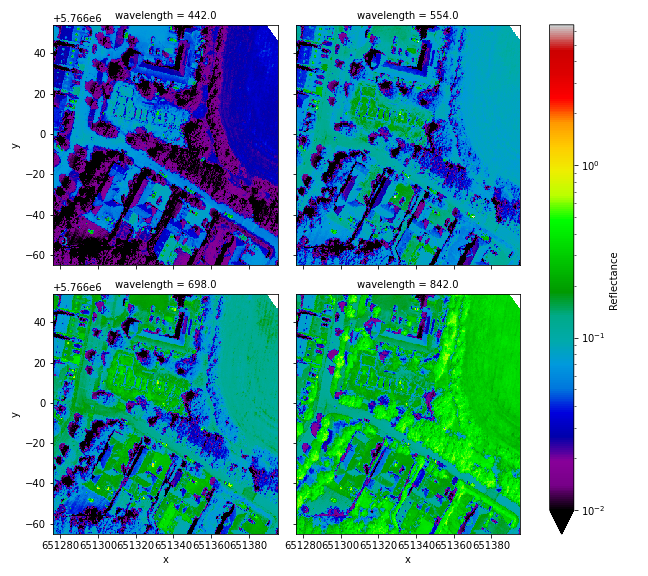
\includegraphics[width=\textwidth]{TreeView_plots/1_input_reflectance.png}
    \caption{Reflectance estimates of a scene over Milton Keynes at 442nm, 554nm, 698nm, 842nm. Colourscale is in log units}
    \label{fig:reflectances1}
\end{figure}

\begin{figure}
    \centering
    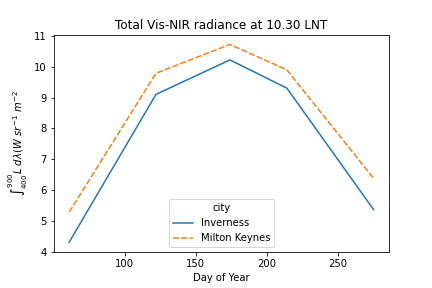
\includegraphics[width=\textwidth]{TreeView_plots/3_integrated_sensor_radiance.png}
    \caption{A. 2D Histogram of reflectance per waveband for the scene in Figure \ref{fig:reflectances1}. Colourscale indicates log pixel count. B. The mean scene radiance (across all pixels) for the same scene, as a function of time (Day of Year) and space (City) using the atmospheric models described above}
    \label{fig:reflectances_hist}
\end{figure}

Reflectance values were converted to at-sensor radiance using the atmospheric models (described in previous section). The mean radiance values across all spatial pixels was integrated w.r.t. wavelength to give the mean radiated signal per unit ground area. This indicated approximately a 1 $W sr^{-1} m^{-2}$ increase in radiance in Milton Keynes compared to Inverness at equivalent Day of Year (Figure \ref{fig:reflectances_hist}.B). Predicted mean radiance values from a lambertian source increased from $4.5 W sr^{-1} m^{-2}$ on the 1st March in Inverness to $10.8 W sr^{-1} m^{-2}$ in Milton Keynes on the 22nd of June.

In order to estimate the measurement range of each band for vegetation signals, the at-sensor radiance values for the scene were masked for vegetation pixels only (NDVI $>$ 0.2). Using all 10 atmospheric scenarios, the 2.5\% and 97.5\% quantiles were retrieved for each spectral band (bandpass responses described in Table \ref{tab:bandpass}) by multiplying the predicted at-sensor radiance values by the spectral response functions (Figure \ref{fig:srfs}). This provided the minimum and maximum expected at-sensor radiance (integrated), for each spectral band.
\begin{table}
\centering
\begin{tabular}{lllll}
\toprule
     & \multicolumn{2}{l}{TreeView v0.1} & \multicolumn{2}{l}{TreeView v0.2} \\
Band & $\lambda$          & FWHM         & $\lambda$          & FWHM         \\
\midrule
0    & 445                & 20           & 440                & 20           \\
1    & 490                & 40           & 480                & 40           \\
2    & 531                & 10           & 525                & 50           \\
3    & 560                & 20           & 585                & 50           \\
4    & 620                & 20           & 630                & 40           \\
5    & 665                & 30           & 670                & 40           \\
6    & 700                & 15           & 700                & 15           \\
7    & 740                & 15           & 740                & 15           \\
8    & 780                & 15           & 780                & 15           \\
9    & 865                & 30           & 865                & 30          \\
\bottomrule
\end{tabular}
    \caption{Bandpass responses in nm for TreeView v0.1 and v0.2}
    \label{tab:bandpass}
\end{table}
\begin{figure}
    \centering
    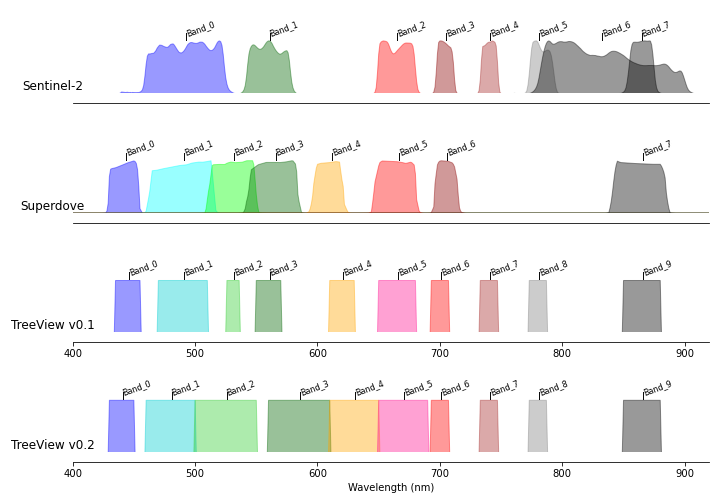
\includegraphics[width=\textwidth]{TreeView_plots/4_sensor_comparison.png}
    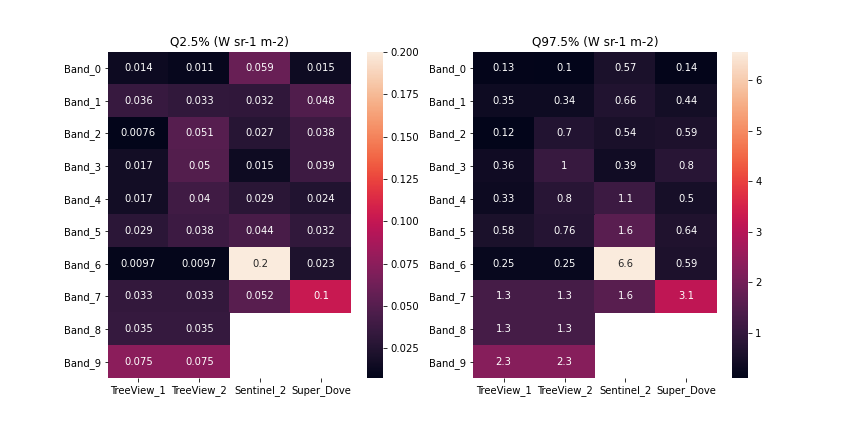
\includegraphics[width=\textwidth]{TreeView_plots/7_minMaxVeg_radiance.png}
    \caption{Estimated 95\% minimum and maximum radiances per spectral band}
    \label{fig:srfs}
\end{figure}
Due to the large range of wavelength-dependent reflectances in the vegetation signal and the differing bandwidths of the proposed TreeView spectral bands, the expected range of radiances across all bands and illumination scenarios was large ($10$--$2300~ mW~sr^{-1}~m^{-2}$, Figure \ref{fig:srfs}). It should be noted that the range only represents diffusing reflectance sources.

\subsection{Sensor Simulation Parameters}
The CIS125 in its proposed configuration has both panchromatic (PAN) and multispectral (MSI) channels, each with two different pixel sub-array lengths (PAN: 16 and 32; MSI: 32 and 64). For the two initial proposed bandpass combinations (v0.1, v0.2), there are therefore 8 sensor configuration combinations to simulate (Table \ref{tab:sim_params}). All simulations fix the swath width at approximately 16Km with a minimum GSD of 2m (MSI channels). A constraint used throughout is a maximum (circular) entrance pupil aperture diameter of 250mm.

\begin{landscape}
\small
\begin{tabular}{lllllllll}
\toprule
{} &  1\_MSI\_16 &  1\_MSI\_32 &  2\_MSI\_16 &  2\_MSI\_32 &  1\_PAN\_32 &  1\_PAN\_64 &  2\_PAN\_32 &  2\_PAN\_64 \\
\midrule
\_fitted                &      True &      True &      True &      True &      True &      True &      True &      True \\
sensor\_altitude        &  500000.0 &  500000.0 &  500000.0 &  500000.0 &  500000.0 &  500000.0 &  500000.0 &  500000.0 \\
sensor\_ground\_speed    &      7000 &      7000 &      7000 &      7000 &      7000 &      7000 &      7000 &      7000 \\
ground\_sample\_distance &         2 &         2 &         2 &         2 &         1 &         1 &         1 &         1 \\
lens\_diameter          &      0.25 &      0.25 &      0.25 &      0.25 &      0.25 &      0.25 &      0.25 &      0.25 \\
psf\_fwhm               &         2 &         4 &         4 &         4 &         2 &         2 &         2 &         2 \\
TDI\_rows               &        16 &        32 &        16 &        32 &        32 &        64 &        32 &        64 \\
pix\_per\_row            &      8196 &      8196 &      8196 &      8196 &     16392 &     16392 &     16392 &     16392 \\
sensor\_width           &      82.2 &      82.2 &      82.2 &      82.2 &      82.2 &      82.2 &      82.2 &      82.2 \\
pixel\_area             &       100 &       100 &       100 &       100 &        25 &        25 &        25 &        25 \\
full\_well              &    106000 &    106000 &    106000 &    106000 &     33000 &     33000 &     33000 &     33000 \\
prnu\_factor            &         0 &         0 &         0 &         0 &         0 &         0 &         0 &         0 \\
dark\_current           &      17.8 &      17.8 &      17.8 &      17.8 &      4.45 &      4.45 &      4.45 &      4.45 \\
dark\_factor            &         0 &         0 &         0 &         0 &         0 &         0 &         0 &         0 \\
offset\_factor          &         0 &         0 &         0 &         0 &         0 &         0 &         0 &         0 \\
ccd\_vref               &         1 &         1 &         1 &         1 &         1 &         1 &         1 &         1 \\
sense\_node\_gain        &      9.43 &      9.43 &      9.43 &      9.43 &      30.3 &      30.3 &      30.3 &      30.3 \\
read\_noise             &        20 &        20 &        20 &        20 &        20 &        20 &        20 &        20 \\
adc\_vref               &         1 &         1 &         1 &         1 &         1 &         1 &         1 &         1 \\
bit\_depth              &        12 &        12 &        12 &        12 &        12 &        12 &        12 &        12 \\
PRNU                   &         0 &         0 &         0 &         0 &         0 &         0 &         0 &         0 \\
DSNU                   &         0 &         0 &         0 &         0 &         0 &         0 &         0 &         0 \\
column\_offset\_FPN      &         0 &         0 &         0 &         0 &         0 &         0 &         0 &         0 \\
integration\_time       &  0.004571 &  0.009143 &  0.004571 &  0.009143 &  0.004571 &  0.009143 &  0.004571 &  0.009143 \\
\_dark\_current          &     284.8 &     569.6 &     284.8 &     569.6 &     142.4 &     284.8 &     142.4 &     284.8 \\
swath\_width            &     16392 &     16392 &     16392 &     16392 &     16392 &     16392 &     16392 &     16392 \\
afov                   &  0.032781 &  0.032781 &  0.032781 &  0.032781 &  0.032781 &  0.032781 &  0.032781 &  0.032781 \\
pix\_width              &   0.00001 &   0.00001 &   0.00001 &   0.00001 &  0.000005 &  0.000005 &  0.000005 &  0.000005 \\
focal\_length           &  2.506647 &  2.506647 &  2.506647 &  2.506647 &  2.506647 &  2.506647 &  2.506647 &  2.506647 \\
\_sense\_node\_gain       &  0.000009 &  0.000009 &  0.000009 &  0.000009 &   0.00003 &   0.00003 &   0.00003 &   0.00003 \\
\bottomrule
\end{tabular}

\end{landscape}

\subsection{Signal-to-Noise Estimation}
Signal-to-Noise ratio was estimated from the simulations for a range of radiance values spanning the expected radiances

\section{Conclusions}
\begin{enumerate}
\item
\end{enumerate}

\bibliography{references}


\end{document}